\documentclass[sigconf]{acmart}

\usepackage{booktabs} % For formal tables

\usepackage{graphicx, url}
\usepackage{balance}
\usepackage{subfigure,wrapfig}
\usepackage{comment}
\usepackage{subfigure, color, colortbl}
\usepackage{amssymb,amsmath}
\usepackage{epstopdf}

%\usepackage{showframe,subcaption,graphicx}
%\usepackage{enumitem}


\newcommand*{\revise}{\textcolor{blue}}
\definecolor{LightCyan}{rgb}{0.0,1,1}
\definecolor{LightGray}{rgb}{0.8,0.8,0.8}

\newcommand*{\edit}{\textcolor{red}}

% Copyright
%\setcopyright{none}
%\setcopyright{acmcopyright}
%\setcopyright{acmlicensed}
\setcopyright{rightsretained}
%\setcopyright{usgov}
%\setcopyright{usgovmixed}
%\setcopyright{cagov}
%\setcopyright{cagovmixed}

%
%% DOI
%\acmDOI{10.475/123_4}
%
%% ISBN
%\acmISBN{123-4567-24-567/08/06}
%
%%Conference
%\acmConference[SenSys'17]{ACM conference}{Nov 2017}{Delft, The Netherlands} 
%\acmYear{1997}
%\copyrightyear{2017}
%
%\acmPrice{15.00}


\begin{document}
\title{Handling Coexistence in LPWAN}

%\titlenote{Produces the permission block, and
%  copyright information}
%\subtitle{Extended Abstract}
%\subtitlenote{The full version of the author's guide is available as
%  \texttt{acmart.pdf} document}


%
%\author{Abusayeed Saifullah}
%\authornote{Co-first author.}
%\affiliation{Wayne State University, Detroit, MI
%%
%%  \institution{The Th{\o}rv{\"a}ld Group}
%%  \streetaddress{1 Th{\o}rv{\"a}ld Circle}
%%  \city{Hekla} 
%%  \country{Iceland}
%  }
%\email{saifullah@wayne.edu}
%
%\author{Mahbubur Rahman}
%\authornotemark[1]
%\affiliation{Wayne State University, Detroit, MI
%%
%%  \institution{The Th{\o}rv{\"a}ld Group}
%%  \streetaddress{1 Th{\o}rv{\"a}ld Circle}
%%  \city{Hekla} 
%%  \country{Iceland}
%  }
%\email{r.mahbub@wayne.edu}
%
%\author{Dali Ismail}
%\affiliation{Wayne State University, Detroit, MI
%%
%%  \institution{The Th{\o}rv{\"a}ld Group}
%%  \streetaddress{1 Th{\o}rv{\"a}ld Circle}
%%  \city{Hekla} 
%%  \country{Iceland}
%  }
%\email{dali.ismail@wayne.edu}
%
%\author{Chenyang Lu}
%\affiliation{Washington University, St Louis, MO
%%  \institution{Brookhaven Laboratories}
%%  \streetaddress{P.O. Box 5000}
%  }
%\email{lu@cse.wustl.edu}
%
%\author{Jie Liu}
%\affiliation{Microsoft Research, Redmond, WA
%%  \institution{NASA Ames Research Center}
%%  \city{Moffett Field}
%%  \state{California} 
%%  \postcode{94035}
%  }
%\email{jie.liu@microsoft.com}
%
%\author{Ranveer Chandra}
%\affiliation{Microsoft Research, Redmond, WA
%%  \institution{NASA Ames Research Center}
%%  \city{Moffett Field}
%%  \state{California} 
%%  \postcode{94035}
%  }
%\email{ranveer@microsoft.com}
%
%\renewcommand{\shortauthors}{A. Saifullah et al.}


\begin{abstract}

 As an emerging Internet-of-Things (IoT) technology, {\slshape Low-Power Wide-Area Network (LPWAN)} enables low-power wireless devices to transmit at low data rates over long distances using narrowband. While many competing LPWAN technologies have been developed recently, they have a number of {\bf major limitations} that make their adoption challenging. Specifically, rapid growth of LPWANs in the limited spectrum raises the challenge of {\bf \underline{coexistence}}.  It will be severe in urban areas where spectrum can be congested due to numerous independent  networks. Due to long range, LPWAN devices can be subject to an unprecedented number of hidden nodes. Today, they are not equipped to handle this impending challenge. It is difficult to employ sophisticated MAC for low-power nodes. We address this challenge in LPWAN by developing theoretical foundations  and systems for {\bf\slshape SNOW (Sensor Network Over White Spaces)}, an LPWAN architecture that exploits the TV white spaces for scalable IoT. Compared to cellular LPWANs, SNOW does not require wired infrastructure making it suitable in both rural and urban areas.  While we focus on SNOW to develop and evaluate the proposed protocols, the approach can be extended to other types of LPWANs for broader impacts on industry. We propose a novel approach based on Reinforcement Learning to handle coexistence with many independent networks.  This is done by developing an efficient  Q-learning framework that is practical at low-power nodes. This will be the {\bf first}  Q-learning approach for LPWAN and for handling coexistence in low-power network. 

\end{abstract}


\begin{CCSXML}
<ccs2012>
<concept>
<concept_id>10003033.10003039</concept_id>
<concept_desc>Networks~Network protocols</concept_desc>
<concept_significance>500</concept_significance>
</concept>
<concept>
<concept_id>10010520.10010553.10003238</concept_id>
<concept_desc>Computer systems organization~Sensor networks</concept_desc>
<concept_significance>500</concept_significance>
</concept>
</ccs2012>
\end{CCSXML}

\ccsdesc[500]{Networks~Network protocols}
\ccsdesc[500]{Computer systems organization~Sensor networks}


\copyrightyear{2017} 
\acmYear{2017} 
\setcopyright{acmcopyright}
\acmConference{SenSys '17}{November 6--8, 2017}{Delft, Netherlands}\acmPrice{15.00}\acmDOI{10.1145/3131672.3131676}
\acmISBN{978-1-4503-5459-2/17/11}

% We no longer use \terms command
%\terms{Theory}

%\keywords{White space, Wireless Sensor Network, LPWAN, OFDM}

\keywords{White space, LPWAN, Sensor Network, OFDM, MAC Protocol.}


\maketitle

 %!TEX root = coexistence_paper.tex


\section{Introduction}\label{sec:introduction}

As an emerging Internet-of-Things (IoT) technology, {\slshape Low-Power Wide-Area Network (LPWAN)} enables low-power (milliwatts) wireless devices to transmit at low data rates (kbps) over long distances (kms) using narrowband (kHz). With the fast growth of IoT, multiple competing LPWAN technologies are currently being developed such as LoRa~\cite{lorawan}, SigFox~\cite{sigfox}, IQRF~\cite{iqrf}, RPMA~\cite{rpma}, DASH7~\cite{dash7}, Weightless-N/P~\cite{weightless}, Telensa~\cite{telensa} in the ISM band,  and  EC-GSM-IoT~\cite{ecgsmiot}, NB-IoT~\cite{nbiot},  LTE Cat M1~\cite{cat, LTE_advancedpro},   5G~\cite{ngmn} in the licensed cellular band. To avoid the {\bf crowd} in the {\bf limited} ISM band and the {\bf cost} of licensed band, we designed {\bf\slshape  SNOW (Sensor Network Over White spaces)}, an LPWAN architecture  to support scalable wide-area IoT  over the TV white spaces \cite{ton_snow, snow, snow2}.  {\slshape White spaces} are the allocated but locally unused TV channels~\cite{FCC_first_order, fcc_second_order}. Compared to ISM band, they have much wider, less crowded spectrum in rural and most urban areas, with an abundance in rural areas 
\cite{ws_sigcomm09}.
 Previously, they were aimed mostly for broadband access by Microsoft~\cite{4Africa, MSRAfrica}, Google~\cite{GoogleAfrica}, standards bodies such as IEEE 802.11af~\cite{IEE802_af},   802.22~\cite{IEEE802_22},   802.19~\cite{IEE802_19}, and in research  
\cite{saeed2017local, ws_dyspan08_kim, ws_mobicom08, ws_dyspan11, FIWEX, dbreq, database1, database2, database3, vehiclebased, hysim, zhang2015design, hasan2014gsm, kumar, harrison2015whitespace, ws_sigcomm09, WATCH, videostreaming, linkasymmetry, ws_mobicom13, ws_nsdi10}. 
Our initial design and experiment showed the potential of SNOW for asynchronous, low power,   massively concurrent communications between numerous nodes and a base station (BS) over long distances, enabling scalable, wide-area IoT in white spaces \cite{ton_snow, snow, snow2}. 




 
Rapid growth of LPWANs in the limited spectrum brings forth the challenge of coexistence.  
The number of connected devices will exceed 50 billions by 2020 \cite{comparativestudylpwan}. 
With Comcast recently announcing to add LPWAN radios on set-top boxes, LPWANs will be ubiquitous in the US~\cite{comcast}. 
Ongoing standardization efforts such as IEEE 802.15.4m \cite{802154m} (extending 802.15.4~\cite{ieee154}) and Weightless-W \cite{weightless} may yield many LPWAN users in white spaces in the future. The coexistence problem will be severe in urban areas where spectrum can be congested due to numerous independent  networks. Today, LPWANs are not equipped to handle this impending challenge~\cite{LPWANSurvey222}. It is difficult to employ sophisticated media access control (MAC) protocol for low-power nodes. Studies show  a collision probability $\approx 1$ if 1000 nodes of LoRa, SigFox, or IQRF coexist \cite{lp1coexistence1, lorascale}. Another study shows significant throughput reduction when four LoRa networks coexist~\cite{voigt2016mitigating}. Coexistence handling for WiFi, traditional short-range wireless sensor network (WSN), and Bluetooth~\cite{survey802154, coexistence_survey, coexistence_24} will not work for LPWANs. Due to long range, their devices are subject to an unprecedented number of hidden nodes, requiring techniques that handle such coexistence while being highly energy-efficient. 



We shall  develop theoretical foundations and systems  to address the above challenges for LPWAN.  Our preliminary work showed advantages of SNOW over other LPWANs in scalability and energy~\cite{snow, snow2, ton_snow}.  It allows the BS to receive concurrent transmissions made by the  nodes asynchronously. It also allows concurrent downlink communication. LoRa relies on time synchronized beacons and schedules for downlink communication.  Compared to cellular LPWANs, SNOW does not need wired infrastructure making it suitable in both rural and urban areas. With the rapid growth of IoT,  LPWANs will suffer from crowded spectrum due to long range, making it  critical to exploit white spaces.  


 We propose a novel approach based on Reinforcement Learning to handle coexistence with many independent networks.  This is done by developing an efficient  Q-learning framework that is practical at low-power nodes. This would be the {\bf first}  Q-learning approach for LPWAN and for handling coexistence for any low-power network. This framework can be adopted for other (non-cellular) LPWANs with minor modification.
 
 
 \revise{The paper is organized as follows. Section \ref{sec:related} describes related work. .........   so on.}



 %!TEX root = coexistence_paper.tex
 \section{Background and System Model}
 We focus on LoRa as an representative LPWAN technologies and handle co-existence for dense LoRa networks with our q-learning framework. In the following sections, we describe the necessary background on LoRa. 
  
 %\subsection{An Overview of SNOW}

 
 %\begin{figure}[!htpb]%{r}{7.3cm}
%\centering\vspace{-0.05in}
%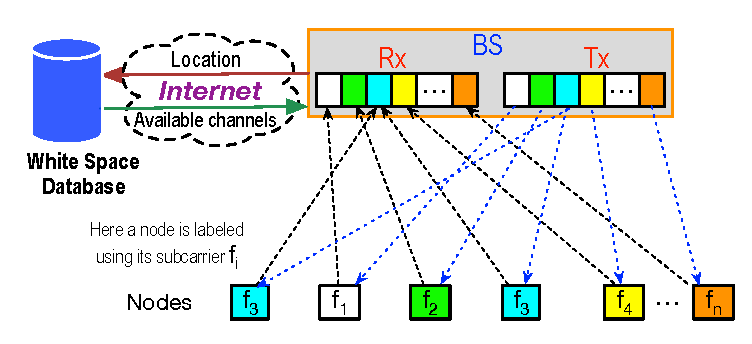
\includegraphics[width=0.44\textwidth]{figs/dual-radio.eps}
%\vspace{-0.1in}
%\caption{\small The SNOW architecture.}
%\label{fig:arch}
%\vspace{-0.1in}
%\end{figure} 
 
 
 %Here we provide a brief overview of the SNOW PHY that we developed previously \cite{snow, snow2, ton_snow}. Its {\bf full description}  is available in~\cite{ton_snow}. Due to long transmission (Tx) range, the nodes in SNOW are directly connected to the BS, forming a star topology as shown in Fig.~\ref{fig:arch}. We use {\bf `node'} to indicate a sensor node.  We assume that the BS knows the locations of the nodes through manual configuration or some existing WSN localization technique~\cite{wsnlocalizationsurvey}. \revise{This assumption is relaxed in our proposed research}. 
%The BS periodically determines white spaces by providing locations of its own and of all other nodes in a cloud-hosted database through the Internet. The BS uses wide white space spectrum as a single wide channel that is split into narrowband orthogonal subcarriers, each of equal spectrum width (bandwidth). Each node has a single half-duplex narrowband radio. It sends/receives on a subcarrier. The nodes are power-constrained, and do not do spectrum sensing or cloud access. As shown in Fig.~\ref{fig:arch}, the BS uses two radios --  one for only transmission (called {\bf\slshape Tx radio})  and the other for only reception (called {\bf\slshape Rx radio}) -- to facilitate concurrent bidirectional communication.  




%
%\begin{figure*}[!htb]
%    \centering\vspace{-0.22in}
%      \subfigure[\footnotesize Node positions in the Detroit metro area\label{fig:outdoor}]{
%	\includegraphics[width=0.37\textwidth]{figs/setup/metro_setup.jpg}
%      }
%    \hfill
%      \subfigure[\footnotesize Uplink reliability\label{fig:reliability_bs_distance}]{
%    \includegraphics[width=0.23\textwidth]{figs/reliability/reliability_bs_distance.eps}
%      }
%      \hfill
%      \subfigure[\footnotesize Distance vs. Tx powers\label{fig:distance_txpower}]{
%        \includegraphics[width=.22\textwidth]{figs/reliability/distance_txpower.eps}
%      }\vspace{-0.2in}
%    \caption{\small Reliability over distances and  varying Tx power.}\vspace{-0.13in}
%    \label{fig:reliability_bs_node}
% \end{figure*}



%A key design goal of SNOW is to achieve high scalability by exploiting wide spectrum of white spaces. Hence, its PHY is designed based on a 
%{\bf D}istributed implementation of {\bf OFDM} for multi-user access, called {\bf D-OFDM}. D-OFDM  splits a wide spectrum into numerous narrowband orthogonal subcarriers enabling parallel data streams to/from numerous distributed nodes from/to the BS.  A subcarrier bandwidth is in kHz (e.g., 50kHz, 100kHz, 200kHz, or so depending on packet size and needed bit rate). Narrower bands have lower bit rate but longer range, and consume less power~\cite{channelwidth}. The nodes transmit/receive on orthogonal subcarriers, each using one. A subcarrier is modulated using Binary Phase Shift Keying (BPSK) or Amplitude Shift Keying (ASK).  If the BS spectrum is split into  $m$  subcarriers,  it can receive from $m$ nodes simultaneously using a single antenna. Similarly, it can transmit different data on different subcarriers through a single transmission. The BS can also use fragmented spectrum. This design is different from MIMO radio adopted in various wireless domains including IEEE 802.11n~\cite{mimo} as they rely on multiple antennas to enable the same. While OFDM has been adopted  for multi-access in the forms of OFDMA  and SC-FDMA in various  broadband (e.g., WiMAX~\cite{wimax}) and cellular  (e.g., LTE~\cite{lte_whitepaper}) technologies~\cite{3gpp, scfdma, OFDMAWiMAX}, they rely on strong time synchronization which is very costly for low-power nodes. We adopted OFDM for the first time in WSN design and without requiring time synchronization. D-OFDM enables multiple packet receptions that are transmitted asynchronously from different nodes which was possible as WSN needs low data rate and short packets. Time synchronization is avoided by extending the symbol duration (repeating a symbol multiple times) and sacrificing bit rate. The effect is similar to extending cyclic prefix (CP) beyond what is required to control  inter-symbol interference (ISI). CPs of adequate lengths have the effect of rendering asynchronous signals to appear orthogonal at the receiver, increasing guard-interval. As it reduces data rate, D-OFDM is suitable for LPWAN. Carrier frequency offset (CFO) is estimated using training symbols when a node joins the network on a subcarrier (right most) whose overlapping subcarriers are not used. Using this CFO, it is  determined on its assigned subcarrier and compensated for using traditional method to mitigate ICI. 



%\begin{figure}%{r}{4cm}
%\centering\vspace{-0.1in}
%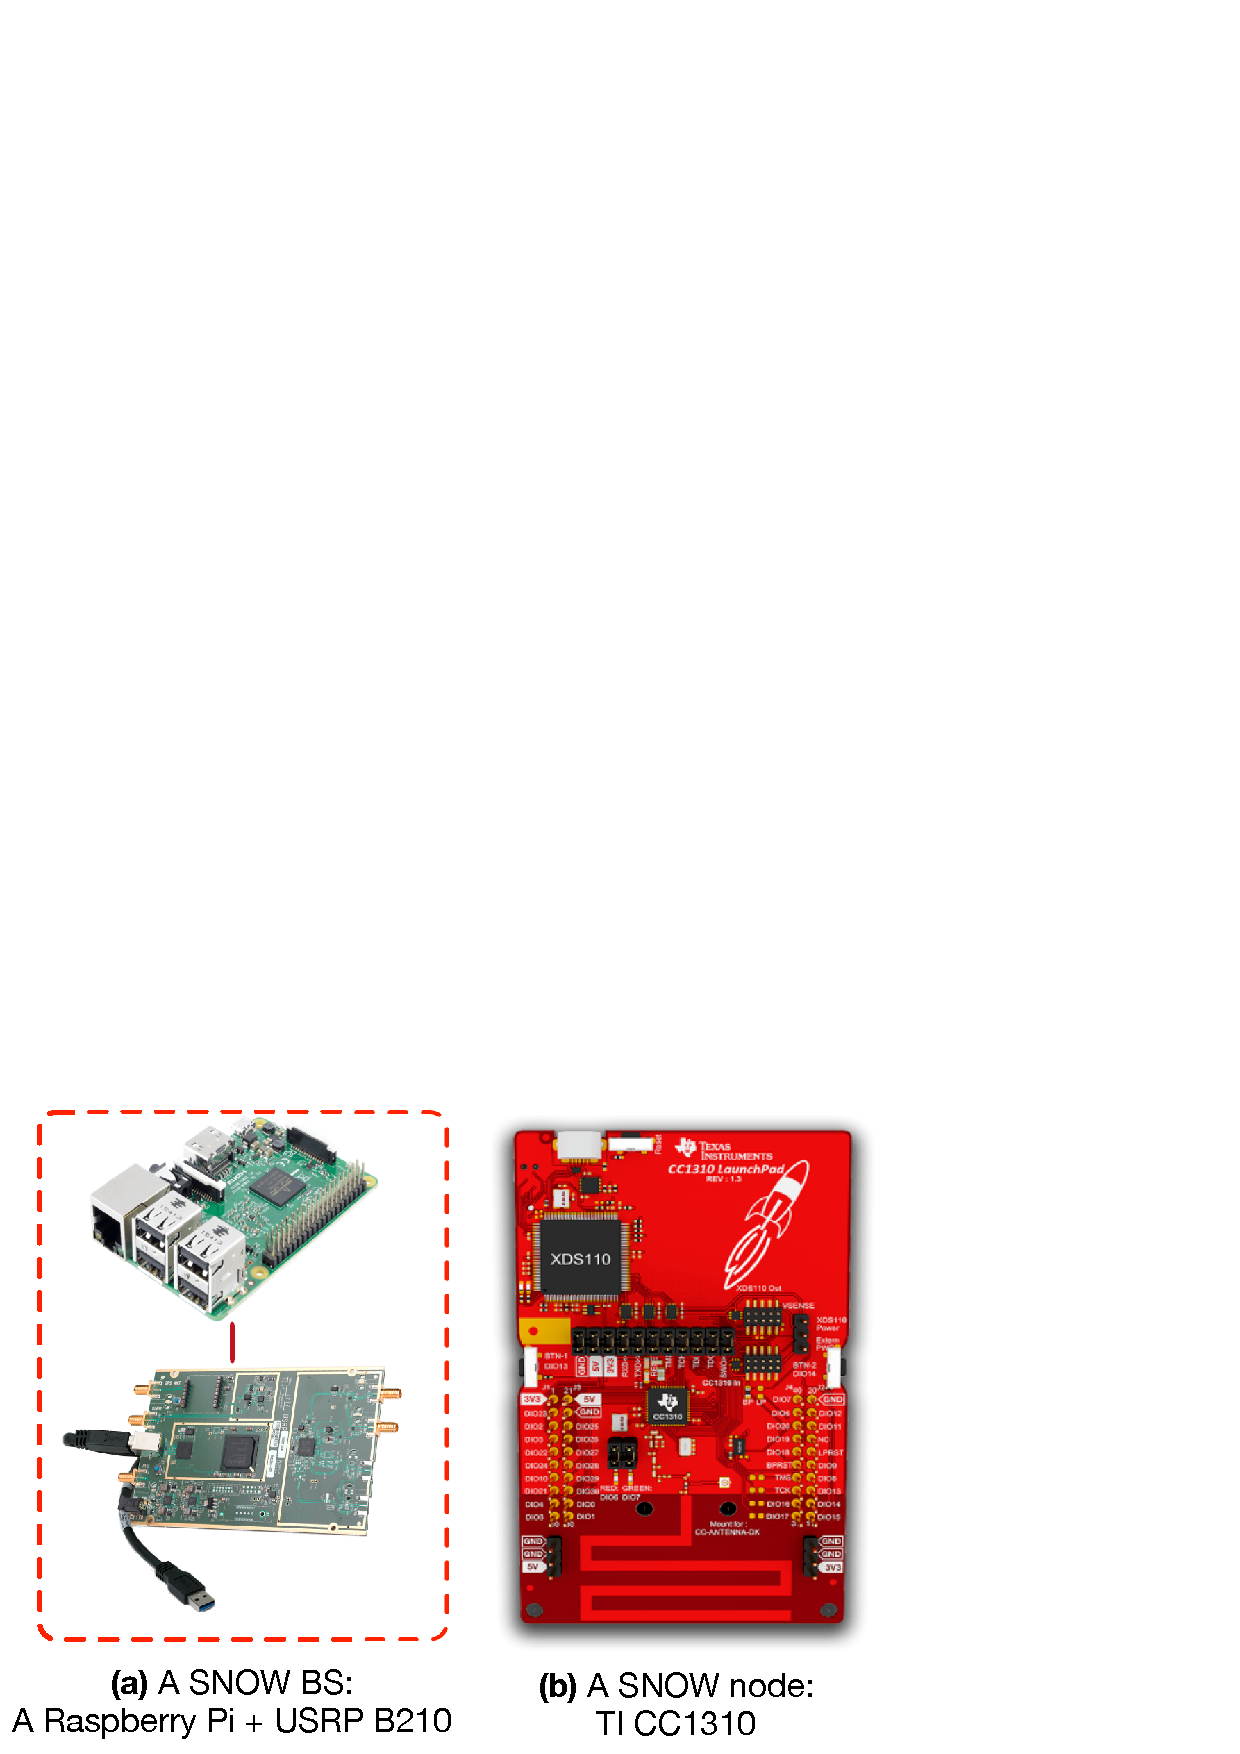
\includegraphics[width=0.34\textwidth]{figs/hardware.jpg}
%\vspace{-0.1in}
%\caption{\footnotesize SNOW Hardware.}
%\label{fig:hardware}
%\vspace{-0.1in}
%\end{figure} 


%We implemented SNOW on two hardware platforms -- USRP~\cite{usrp} using GNU radio~\cite{gnuradio} and TI CC1310~\cite{cc1310}. 
%Using a simple CSMA/CA based MAC protocol, our preliminary experiments showed its better scalability and energy efficiency over other LPWANs~\cite{snow, snow2, ton_snow}.  \revise{We observed a Tx range of 8km at 20dBm.}    
%CC1310 is a tiny, cheap ($<$\$30), and commercially off-the-shelf (COTS) device with a programmable PHY. 
%We implemented SNOW with CC1310 (using CC-ANTENNA-DK2)  as a SNOW node (Fig. \ref{fig:hardware} (a)) \cite{snowdemo}. The BS is a USRP210 with a laptop (Fig. \ref{fig:hardware} (b)). Since CC1310 allows us to use ASK modulation and up to 15dBm Tx power, we achieved 1.5km Tx range compared to 8km achieved using USRP. We have set a testbed using both USRP and CC1310 devices as SNOW nodes \cite{opensource}.  As the frequencies of SNOW's operating spectrum  are close to that (lower ISM band) of most LPWANs, its antenna form factor will be close to those in real production. 


\subsection{An Overview of LoRa}
\revise{Here we provide a brief overview of LoRa(Long-Range). Detailed description for the physical and link-layer of LoRa networks can be found in~\cite{LoRaWAN_spec_v1.1}. LoRa is the physical layer technology for an LPWAN. It's characteristics include extremely long-range which can be in the range of 3-7 miles depending on the environment and successful reception of packets even at extremely low signal-to-noise ratio. LoRa modulation is derived from \emph{Chirp Spread Spectrum (CSS)}. CSS modulation spreads the signal over the entire bandwidth, thus providing robustness to interference and enabling reception of packet at very low signal-to-noise ratio. The modulated signal consists of symbols/chirps, whose frequency linearly increases or decreases over time. Information is encoded onto each chirp using multiple cyclic shifted chips. The number of chips present in each symbol is controlled by the \emph{spreading factor}. Specifically, spreading factor is the ratio between symbol rate and chip rate. LoRa supports spreading factor in the range [6,12]. Spreading factor (SF) controls the data rate and thus the transmission time and energy consumption. A higher spreading factor reduces the data rate and thus increases the time on air for each packet leading to significant increase in energy consumption.  Transmissions on different spreading factors are orthogonal to each other. }

\revise{LoRa also supports different levels of forward error detection (FEC), called \emph{coding rates} in the range of $\frac{4}{5}$ to $\frac{4}{8}$ A higher coding rate provides resilience against bursts of interference, but increases the duration of each packet. Apart from coding rate and spreading factor, other configurable parameters for LoRa are carrier frequency, channel and bandwidth. Carrier frequency and channels vary from region to region depending on local regulation. For example, in the US band LoRa operates in the range 902-928MHz. For uplink communication in the US, there are 64 channels of bandwidth 125kHz and 8 channels of bandwidth 500kHz. For downlink, there are 8 channels of bandwidth 500kHz. }

\revise{The MAC protocol used with LoRa physical layer is called LoRa Wide Area Network(LoRaWAN). In LoRaWAN numerous nodes are directly connected to one of more gateways, which forward the data collected from nodes to a central network server. Thus, LoRa forms a star of star network topology. LoRaWAN supports classes of operation, namely class A,B and C. In all classes, nodes transmit using pure ALOHA. In class A, nodes transmit when they have data and open two receive windows after each transmission. In class B, gateway send periodic beacons to synchronize nodes. Between two beacons, the nodes wake up periodically to receive any packets from the gateway. In class C, the nodes are continuously listening for packets from the gateway.}
 
\subsection{System Model}
\revise{We consider LPWAN networks consisting of numerous nodes connected directly to one or more gateways. We consider a dense deployment where multiple LPWAN networks are operating in the same spectrum. We assume that the nodes and gateways of these networks do not posses any knowledge about each other and operate independently. Nodes are battery-powered and only wake-up if they have data to send. Nodes do not posses significant computing power and memory. Gateways are line-powered devices and are always active. We assume that the gateways can support concurrent receptions of multiple packets up to some limit. Thus, the gateways are limited by maximum number of simultaneous receptions $n$ which can be controlled by the network manager. If more than $n$ packets arrive at the gateway at the same time, some packets are dropped. Nodes rely on acknowledgements from the gateway to confirm successful reception of data. Nodes retransmit the packet if an acknowledgement is not received. The maximum number of retransmissions is also configured by the network manager.}
 %!TEX root = coexistence_paper.tex


 
 \section{Related Work and New Challenges} 
Limited power budget of LPWAN nodes makes it difficult to adopt sophisticated MAC.   
Hence, SigFox and LoRa resort to ALOHA~\cite{tanenbaum} with no collision avoidance.  SNOW currently uses a lightweight CSMA/CA approach. While such lightweight protocols provide energy efficiency, they cannot handle coexistence while low-power transmissions are easily subject to interference.  Coexistence study through simulations revealed that using multiple gateways in distant places can improve some throughput in LoRa~\cite{voigt2016mitigating}. This trivial approach needs more infrastructure support and cost while the gain is marginal. {\slshape Choir} \cite{Choir} is a reactive and PHY-layer approach for handling dense deployment of LoRa in urban areas which leverages on resolving the collided packets. In an uncoordinated environment where packets from many unknown networks can collide, such an approach will not work. The study in \cite{ICC_coexistence}  uses Poisson cluster process to model LoRa dense networks but does not propose coexistence handling. 
While there exists much work on wireless coexistence considering WiFi, WSN, and Bluetooth (see  surveys~\cite{survey802154, coexistence_survey, coexistence_24}), it will not work well for LPWANs. Due to their large coverage domains, LPWAN devices can be subject to an unprecedented number of hidden terminals. 
With their rapid growth while the spectrum is limited, coexistence will be a severe problem and new techniques that are both energy efficient and capable of handling coexistence must be developed. 

 %!TEX root = coexistence_paper.tex



\section{Handling Coexistence}\label{sec:coexistence}
  


 

In massive crowds of coexisting networks, the interference pattern can be hard to detect for an LPWAN device like LoRa .  Hence, a TDMA (time division multiple access) or traditional CSMA/CA based approach will simply fail. As the wireless environment is largely unknown due to the coexistence of a massive number of unknown devices/networks,  a {\slshape learning} based approach becomes more effective to make actions (e.g, transmit, sleep, backoff) according to the environmental conditions. However, a learning process usually can be time and computation extensive while the nodes are power-constrained and battery-operated. Hence, we propose to adopt a lightweight machine learning approach. Specifically, as the SNOW nodes may have no knowledge of the coexisting networks, we will adopt  {\bf\slshape Reinforcement Learning (RL)} that enables an {\slshape agent} (e.g., a node) to learn by interacting with its environment~\cite{RLBook}. As shown in Fig.~\ref{fig:reinforcement}, an agent regularly updates its achieved {\slshape rewards} based on the taken action at a given {\slshape state}.  It will learn to take the best actions that maximize its long-term rewards by using its own experience. This would be the {\bf first RL approach} for LPWAN and for handling coexistence for any low-power network. 



 
    \begin{figure}%{r}{4.2cm}
    \centering%\vspace{-0.6in}
    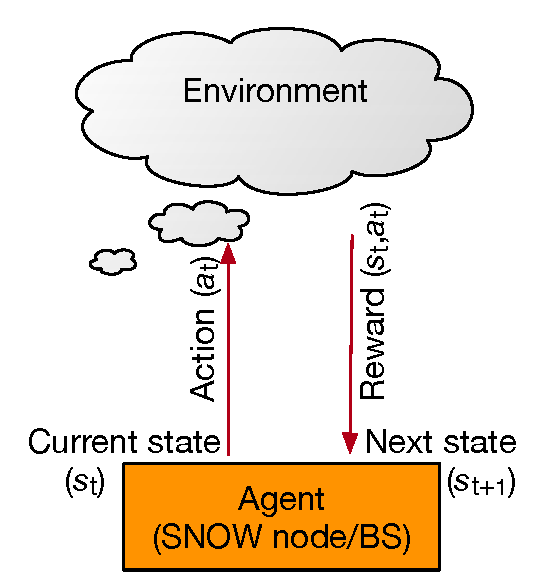
\includegraphics[width=0.22\textwidth]{figs/reinforcement.eps}      
    \vspace{-0.05in}
    \caption{\scriptsize RL visualization}\vspace{-0.1in}
    \label{fig:reinforcement}
 \end{figure}
 
 
\subsection{Rationale for Reinforcement Learning} 
 We adopt {\slshape Q-learning},  a widely-adopted RL technique, which is well-suited for coexistence handling because it is useful in decision making under unknown network conditions. It has {\slshape low memory requirements} and {\slshape low computation}, and learns  near-optimal or even {\slshape optimal} solution under certain conditions. Q-learning can be {\slshape efficiently} implemented in a distributed platform like WSN, where each node chooses actions to maximize rewards. It has been efficiently used in cognitive radios~\cite{cognitive1}, and in WSN for routing~\cite{RLRouting1, RLRouting2, RLRouting3, RLRouting4},  QoS provisioning~\cite{QoS1, QoS2}, and resource management \cite{RLSurvey}. It was also used with  RTS/CTS  to learn contention and collision with the nodes in the {\bf same} network  using a {\bf single channel}~\cite{RLMAC}.  SNOW exploits many subcarriers concurrently and does not rely on energy-consuming RTS/CTS frames. We aim to adopt RL to handle its coexistence with numerous  unknown and uncoordinated networks. RL has not yet been adopted to handle such coexistence. LPWAN technologies like LoRa or SNOW have unique features which require a new Q-learning framework. For example, LoRa networks enable multiple concurrent transmissions by dynamically adjusting multiple transmission parameters, whereas SNOW features massive concurrent communications on numerous narrowband subcarriers, white space dynamics, and PAPR constraints. Our Q-learning framework is able to dynamically leverage each of these unique characteristics to effectively handle co-existance. 
 
 
 %Adopting it for SNOW that features massive concurrent communications on numerous narrowband subcarriers, white space dynamics, PAPR constraints, and very low-power requires a new  Q-learning framework. 
   
%\subsection{Proposed Q-Learning Framework for SNOW}

%SNOW nodes will adopt Q-learning. The purpose of learning in nodes is to learn about the communication pattern of the coexisting networks. 
%On the BS side, this can help determine usable subcarriers and their use pattern.  The actions of a BS can also include load balancing among the subcarriers considering its outside utilization (in coexisting users). 
%To each node, we assign  prioritized access to multiple subcarriers. The intuition is that if one subcarrier is busy or noisy, another may remain free.
%A node will  start with its first priority subcarrier. If a subcarrier is busy,  it will either back-off or hop to its next subcarrier. If Tx fails on one subcarrier, a node can choose to retransmit on the same or the next prioritized subcarrier on a higher Tx power.  When a node has chosen a subcarrier it can either transmit on it, or backoff, or hop to the next priority subcarrier, or sleep. If some subcarriers become unavailable due to primary users, the nodes are informed using some backup subcarriers which is a common technique  in cognitive radios~\cite{ws_sigcomm09}. \revise{Nodes switch to backup subcarriers if no communication happens on their subcarriers for a certain time length.}  Since the BS can use fragmented spectrum, it can turn on and off some subcarriers based on their noise level. The Q-learning framework on the BS side will take into account the cost associated with PAPR in downlink communication. To reduce PAPR, it uses a subset of the Rx subcarriers on the Tx radio for sending ACKs. A node may need to transmit on one subcarrier and listen for ACK on another. The BS may put multiple ACKs on a subcarrier along with any subcarrier reassignment information. 


%    \begin{figure}%{r}{4.2cm}
  %  \centering%\vspace{-0.6in}
 %   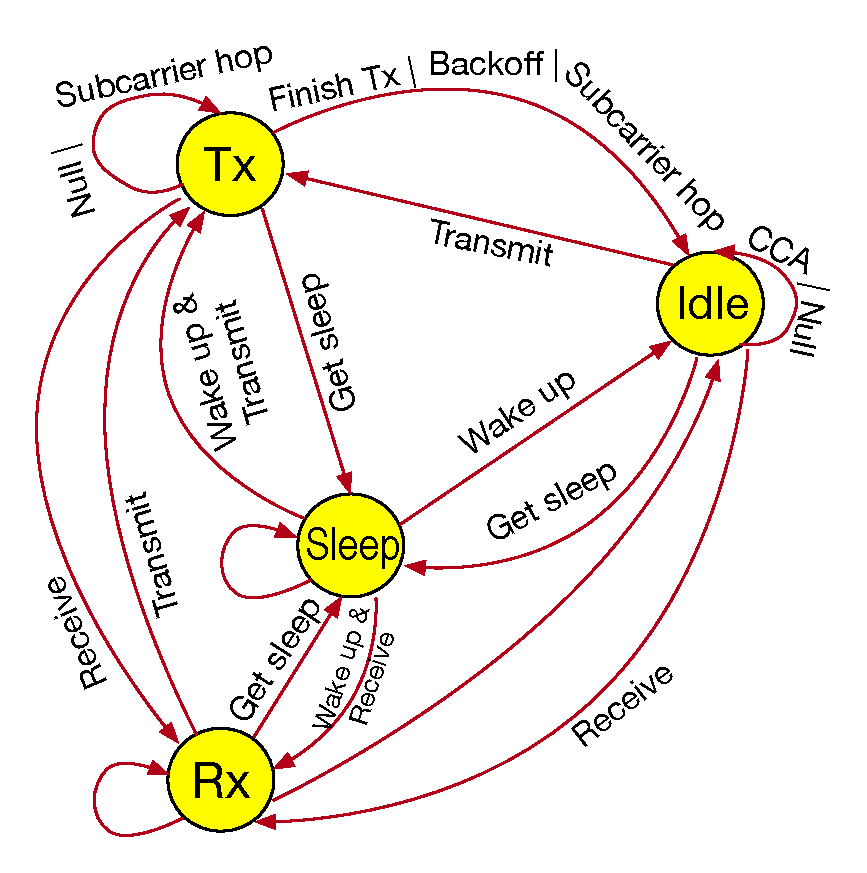
\includegraphics[width=0.33\textwidth]{figs/statediagram.eps}      
 %   \vspace{-0.05in}
 %   \caption{\scriptsize Agent state diagram}\vspace{-0.1in}
 %   \label{fig:statediagram}
%\end{figure}


%\noindent{\bf Reward Function Formulation for Node.}  Every SNOW node individually adopts Q-learning to make its decision. It adopts 
%{\slshape CCA (clear channel assessment)} for carrier sensing. Its set of actions is $\Lambda= \{ \text{\slshape \small Transmit, Receive, Backoff, Wake up, Subcarrier hop, CCA, Get sleep, null} \}$. We  consider agent (node) states $\Omega=\{\text{\slshape \small Tx, Rx, Idle, sleep}  \}$, to indicate its state of transmitting, receiving, idle,  sleeping.   Fig.~\ref{fig:statediagram} shows state transitions. Let $s_t\in \Omega$  be the agent state at time $t$. Its total reward is given by 
 % \vspace{-2mm}
 %$$
% \vspace{-2mm}
% R(s_t, a_t) = r(s_t, a_t) + c(s_t, a_t),$$
% where $r(s_t, a_t)$ is the {\slshape immediate reward}  and $c(s_t, a_t)$ is the {\slshape cost} of taking action $a_t\in \Lambda$  at state $s_t$. Considering both energy consumption and throughput, we can assign some numerical values indicating rewards and costs. As an example, we can consider total reward for a successful packet {\slshape transmission} or {\slshape reception} by considering 2 units of immediate reward  and 1 unit of cost. Thus, a failed transmission will incur only a cost of 1 unit. We can also consider 1 unit of cost in {\slshape idle} state (as the radio consumes energy almost similar to Tx/Rx). From $s_t=${\slshape Idle}, important reward functions can be given as follows. 
%\begin{footnotesize}

%$$%\vspace{-1mm}
%R(s_t, a_t) =
%\begin{cases}
%2 - 1 = 1   & \text{if }  s_t= \text{\slshape Idle},     ~a_t= \text{{\slshape Transmit} and ACK received}\\
%0 - 1 = -1   & \text{if } s_t= \text{\slshape Idle},     ~a_t= \text{{\slshape Transmit} and ACK not received}\\
%2 - 1 = 1   & \text{if } s_t= \text{\slshape Idle},     ~a_t= \text{\slshape Receive}\\
%- 1   & \text{if } s_t= \text{\slshape Idle},     ~a_t= \text{\slshape Null}\\
%- 1   & \text{if } s_t= \text{\slshape Idle},     ~a_t= \text{\slshape CCA}\\
%0   & \text{if } s_t= \text{\slshape Idle},     ~a_t= \text{\slshape Get sleep}
%\end{cases}
%$$\end{footnotesize}
%\revise{
%\begin{footnotesize}
%$$%\vspace{-1mm}
%R(s_t, a_t) =
%\begin{cases}
%2 - 1 = 1   & \text{if }  s_t= \text{\slshape Sleep},     ~a_t= \text{{\slshape Transmit} and ACK received}\\
%0 - 1 = -1   & \text{if } s_t= \text{\slshape Sleep},     ~a_t= \text{{\slshape Transmit} and ACK not received}\\
%2 - 1 = 1   & \text{if } s_t= \text{\slshape Sleep},     ~a_t= \text{\slshape Receive}\\
% 0   & \text{if } s_t= \text{\slshape Sleep},     ~a_t= \text{\slshape Null}\\
%-1   & \text{if } s_t= \text{\slshape Sleep},     ~a_t= \text{\slshape Wake up}
%\end{cases}
%$$\end{footnotesize}
%}

%\revise{
%\begin{footnotesize}
%$$%\vspace{-1mm}
%R(s_t, a_t) =
%\begin{cases}
%2 - 1 = 1   & \text{if }  s_t= \text{\slshape Tx},     ~a_t= \text{{\slshape Finish Tx} and ACK received}\\
%0 - 1 = -1   & \text{if } s_t= \text{\slshape Tx},     ~a_t= \text{{\slshape Finish Tx} and ACK not received}\\
%- 1   & \text{if } s_t= \text{\slshape Tx},     ~a_t= \text{{\slshape Backoff}}\\
%- 1   & \text{if } s_t= \text{\slshape Tx},     ~a_t= \text{{\slshape Subcarrier hop and remain Idle}}\\
%2 - 1 = 1   & \text{if } s_t= \text{\slshape Tx},     ~a_t= \text{{\slshape Subcarrier hop, transmit and ACK received}}\\
%- 1 = 1   & \text{if } s_t= \text{\slshape Tx},     ~a_t= \text{{\slshape Subcarrier hop, transmit and ACK not received}}\\
%2 - 1 = 1   & \text{if } s_t= \text{\slshape Tx},     ~a_t= \text{\slshape Receive}\\
%-1   & \text{if } s_t= \text{\slshape Tx},     ~a_t= \text{\slshape Null}\\
%0   & \text{if } s_t= \text{\slshape Tx},     ~a_t= \text{\slshape Get %Sleep}
%\end{cases}
%$$\end{footnotesize}
%}
%\revise{
%\begin{footnotesize}
%$$%\vspace{-1mm}
%R(s_t, a_t) =
%\begin{cases}
%2 - 1 = 1   & \text{if }  s_t= \text{\slshape Rx},     ~a_t= \text{{\slshape Finish Rx}}\\
%2 - 1 = 1   & \text{if } s_t= \text{\slshape Rx},     ~a_t= \text{{\slshape Transmit} and ACK received}\\
%0 - 1 = - 1   & \text{if } s_t= \text{\slshape Rx},     ~a_t= \text{{\slshape Transmit} and ACK not received}\\
%- 1   & \text{if } s_t= \text{\slshape Rx},     ~a_t= \text{{\slshape go to idle}}\\
%-1   & \text{if } s_t= \text{\slshape Rx},     ~a_t= \text{\slshape Null}\\
%0   & \text{if } s_t= \text{\slshape Rx},     ~a_t= \text{\slshape Get Sleep}
%\end{cases}
%$$\end{footnotesize}}
%\noindent \revise{Based on this idea, we need to formulate  all reward functions for a node agent...... }



%\noindent{\bf Reward Function Formulation for BS.} Here we provide an outline to formulate reward functions for the BS. 
%The BS will maintain states and actions for each subcarrier on both Rx radio and the Tx radio. For our preliminary formulation, we consider two states, Rx\_OFF and Rx\_ON, for each subcarrier on the Rx radio to indicate if it is ON or OFF. The actions are: {\slshape Turn Rx ON}, {\slshape Turn Rx OFF}, and {\slshape null}. We consider similar states and actions for each subcarrier on the Tx radio. A state diagram showing these states and actions is shown in Fig.~\ref{fig:sc_statediagram} for a subcarrier at the BS. For a subcarrier $f_i$ used in the Rx radio for receiving from the nodes, let {\bf rps}$(t,i)$ be packet rate (number of packets received per unit time) per subcarrier at time $t$ if we add subcarrier $f_i$ to the Rx radio.  Let {\bf lps}$(t,i)$ be loss rate (number of times the BS recognizes high signal strength on a subcarrier but cannot decode packet per unit time) per subcarrier at time $t$ if we add subcarrier $f_i$ to the Rx radio. Thus, rps$(t,i)$ and lps$(t,i)$ can be considered {\slshape reward} and {\slshape cost}, respectively, for turning $f_i$ on at the Rx radio. Let {\bf aps}$(t,i)$ be ACK rate (number of ACKs sent per unit time) per subcarrier at time $t$ if we add subcarrier $f_i$ to the Tx radio. Let $m_{\text{tx}} (t)$ be the total number of subcarriers used by the Tx radio for ACK at time $t$. If the BS's maximum tolerable PAPR is $\beta$, then if adding a subcarrier  exceeds this value, i.e.  if $m_{\text{tx}} (t)+1 > \beta$, we  consider a penalty (cost) as the BS has to dissipate more energy. Considering $\nu$ as some normalized cost per subcarrier,   R-values for subcarrier $f_i$ can be formulated as follows.





%\begin{small}
$$
%R(s^i_t, a^i_t) =
%\begin{cases}
%\text{rps} (t, i) - \text{lps} (t, i)  & \text{if }  s^i_t= \text{\slshape Rx\_OFF},     ~a^i_t= \text{{\slshape Turn Rx ON}}\\
%\text{aps} (t, i)   -     \frac{\max \big (0,   m_{\text{tx}} (t) +1  - \beta \big )}{\beta}   & \text{if }  s^i_t= \text{\slshape Tx\_OFF},     ~a^i_t= \text{{\slshape Turn Tx ON}}
%\text{aps} (t, i)   -   \nu . \max \big (0,   m_{\text{tx}} (t) +1  - \beta \big )  & \text{if }  s^i_t= \text{\slshape Tx\_OFF},     ~a^i_t= \text{{\slshape Turn Tx ON}}
%\end{cases}
$$
%\end{small}

%\noindent{\bf Reward Function Formulation for LoRa node.}
%to do..(may remain the same with snow node)

%\noindent{\bf Reward Function Formulation for LoRa BS.}
%LoRa gateways are half-duplex. Thus they can not receive and transmit at the same time. Moreover, a LoRa gateway can only transmit to an end device if it has received a transmission from it. If a LoRa gateway turns its transmission 
%\begin{small}
%$$
%R(s^i_t, a^i_t) =
%\begin{cases}
%\text{rps} (t, i) - \text{lps} (t, i)  & \text{if }  s^i_t= \text{\slshape TX\_ON},     ~a^i_t= \text{{\slshape Turn Rx ON}}\\
%\text{aps} (t, i)   -     \frac{\max \big (0,   m_{\text{tx}} (t) +1  - \beta \big )}{\beta}   & \text{if }  s^i_t= \text{\slshape Tx\_OFF},     ~a^i_t= \text{{\slshape Turn Tx ON}}
%\text{aps} (t, i)   -   \text{mps}(t,i)  & \text{if }  s^i_t= \text{\slshape Rx\_ON},     ~a^i_t= \text{{\slshape Turn Tx ON}}
%\end{cases}
%$$
%\end{small}


 
\subsection{Proposed Q-learning \edit{Frame work} for LoRa}
LoRa nodes will use Q-learning MAC for uplink communication. The Q-learning MAC aims to learn the communication pattern of other co-existing networks and take intelligent decisions to increase the network performance. Each node will start transmitting on a randomly selected channel from the set of enabled channels in the operating band. The network manager initially assigns spreading factors to nodes. Nodes start transmitting using the allocated spreading factors. However, nodes can change their channel and spreading factor after each transmission based on the Q-learning MAC. After each failed transmission,the nodes can choose to transmit in another channel, or transmit using another spreading factor or they can choose to not re-transmit immediately and back-off. 

 \begin{figure*}%[!htpb]%{r}{4.1cm}
    \centering%\hfill
    \subfigure[\footnotesize SNOW Node states\label{fig:statediagram}]{
     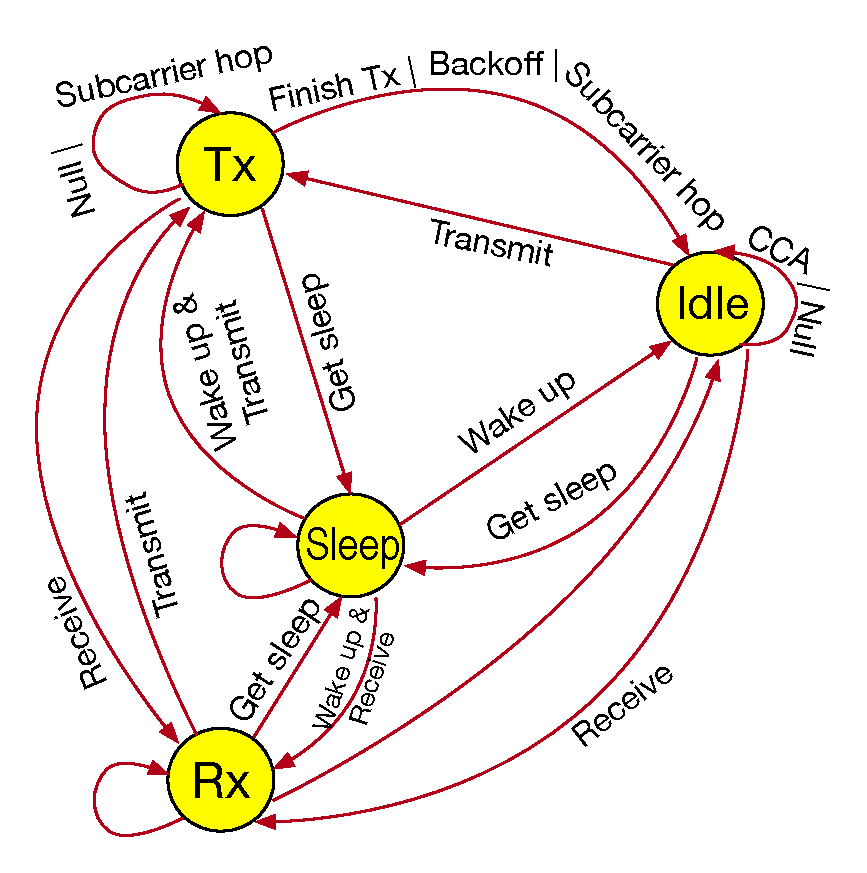
\includegraphics[width=.33\textwidth]{figs/statediagram.eps}
    } \hfill
    \subfigure[\footnotesize LoRa Node States states.\label{fig:statediagram_lora}]{
    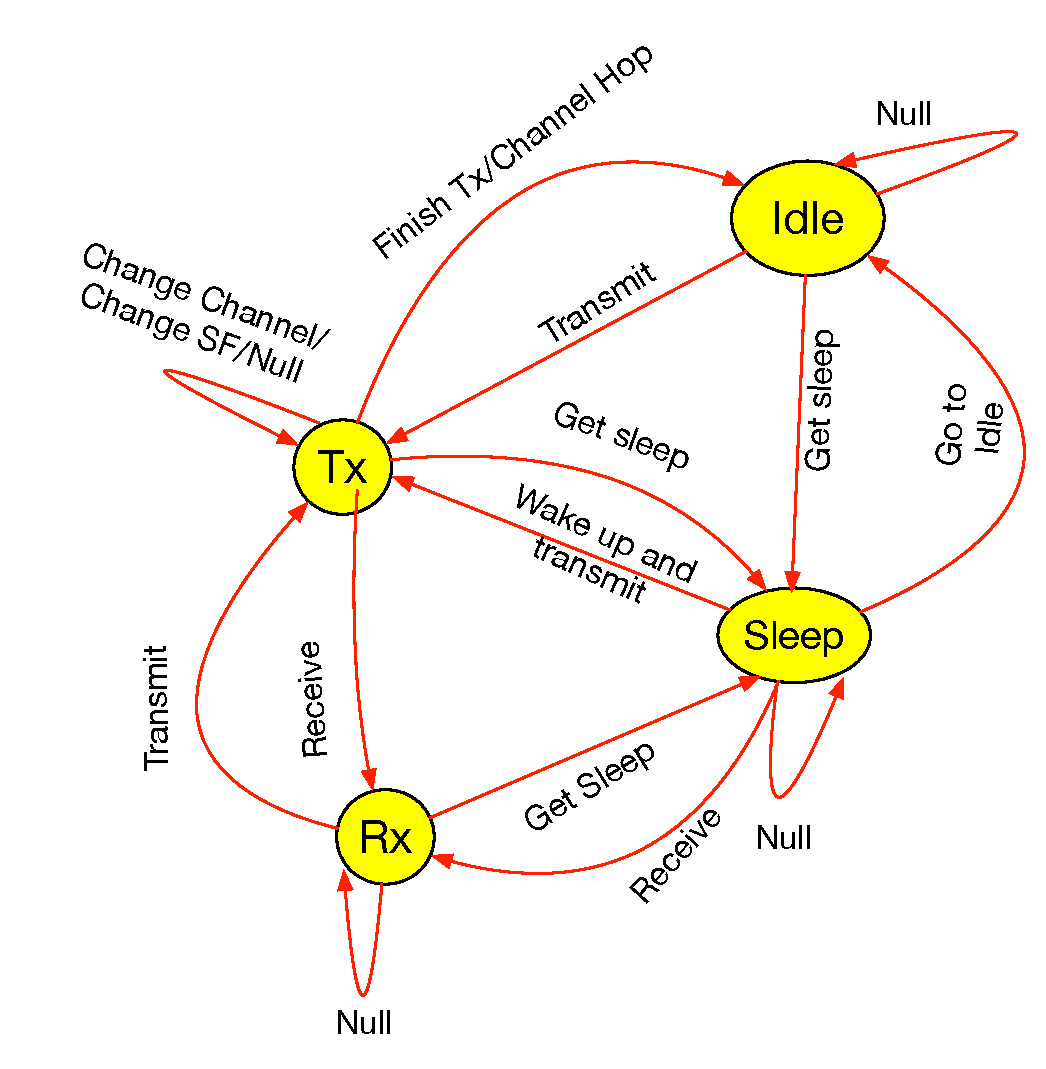
\includegraphics[width=0.4\textwidth]{figs/State_diagram_lora.eps}
      }
      \vspace{-0.15in}
    \caption{\footnotesize Agent state diagram.}%\vspace{-.15in}
   \label{fig:rl}
 \end{figure*}
 
 
Thus, the set of actions is
\vspace{-2mm}
 $$
  \vspace{-2mm}
  \Lambda=\{\text{\slshape \small Transmit, Receive, Backoff, Wake up, Channel hop, Change SF, Get sleep, null}\}$$
 We  consider agent (node) states $\Omega=\{\text{\slshape \small Tx, Rx, Idle, sleep}  \}$, to indicate its state of transmitting, receiving, idle,  sleeping. Based on this action set, the reward functions for LoRa nodes can be constructed as follows: 


\revise{
\begin{footnotesize}
$$%\vspace{-1mm}
R(s_t, a_t) =
\begin{cases}
2 - 1 = 1   & \text{if }  s_t= \text{\slshape Idle},     ~a_t= \text{{\slshape Transmit} and ACK received}\\
0 - 1 = -1   & \text{if } s_t= \text{\slshape Idle},     ~a_t= \text{{\slshape Transmit} and ACK not received}\\
2 - 1 = 1   & \text{if } s_t= \text{\slshape Idle},     ~a_t= \text{\slshape Receive}\\
- 1   & \text{if } s_t= \text{\slshape Idle},     ~a_t= \text{\slshape Null}\\
0   & \text{if } s_t= \text{\slshape Idle},     ~a_t= \text{\slshape Get sleep}
\end{cases}
$$\end{footnotesize}
}

\revise{
\begin{footnotesize}
$$%\vspace{-1mm}
R(s_t, a_t) =
\begin{cases}
2 - 1 = 1   & \text{if }  s_t= \text{\slshape Sleep},     ~a_t= \text{{\slshape Transmit} and ACK received}\\
0 - 1 = -1   & \text{if } s_t= \text{\slshape Sleep},     ~a_t= \text{{\slshape Transmit} and ACK not received}\\
2 - 1 = 1   & \text{if } s_t= \text{\slshape Sleep},     ~a_t= \text{\slshape Receive}\\
 0   & \text{if } s_t= \text{\slshape Sleep},     ~a_t= \text{\slshape Null}\\
-1   & \text{if } s_t= \text{\slshape Sleep},     ~a_t= \text{\slshape Wake up}
\end{cases}
$$\end{footnotesize}
}

\revise{
\begin{footnotesize}
$$%\vspace{-1mm}
R(s_t, a_t) =
\begin{cases}
2 - 1 = 1   & \text{if }  s_t= \text{\slshape Tx},     ~a_t= \text{{\slshape Finish Tx} and ACK received}\\
0 - 1 = -1   & \text{if } s_t= \text{\slshape Tx},     ~a_t= \text{{\slshape Finish Tx} and ACK not received}\\
- 1   & \text{if } s_t= \text{\slshape Tx},     ~a_t= \text{{\slshape Backoff}}\\
- 1   & \text{if } s_t= \text{\slshape Tx},     ~a_t= \text{{\slshape Channel hop and remain Idle}}\\
2 - 1 = 1   & \text{if } s_t= \text{\slshape Tx},     ~a_t= \text{{\slshape Channel hop, transmit and ACK received}}\\
- 1 = 1   & \text{if } s_t= \text{\slshape Tx},     ~a_t= \text{{\slshape Channel hop, transmit and ACK not received}}\\
2 - 1 = 1   & \text{if } s_t= \text{\slshape Tx},     ~a_t= \text{{\slshape Change SF, transmit and ACK received}}\\
- 1 = 1   & \text{if } s_t= \text{\slshape Tx},     ~a_t= \text{{\slshape Change SF, transmit and ACK not received}}\\
-1   & \text{if } s_t= \text{\slshape Tx},     ~a_t= \text{\slshape Null}\\
0   & \text{if } s_t= \text{\slshape Tx},     ~a_t= \text{\slshape Get Sleep}
\end{cases}
$$\end{footnotesize}
}
\revise{
\begin{footnotesize}
$$%\vspace{-1mm}
R(s_t, a_t) =
\begin{cases}
2 - 1 = 1   & \text{if }  s_t= \text{\slshape Rx},     ~a_t= \text{{\slshape Finish Rx}}\\
2 - 1 = 1   & \text{if } s_t= \text{\slshape Rx},     ~a_t= \text{{\slshape Transmit} and ACK received}\\
0 - 1 = - 1   & \text{if } s_t= \text{\slshape Rx},     ~a_t= \text{{\slshape Transmit} and ACK not received}\\
- 1   & \text{if } s_t= \text{\slshape Rx},     ~a_t= \text{{\slshape go to idle}}\\
-1   & \text{if } s_t= \text{\slshape Rx},     ~a_t= \text{\slshape Null}\\
0   & \text{if } s_t= \text{\slshape Rx},     ~a_t= \text{\slshape Get Sleep}
\end{cases}
$$\end{footnotesize}}

 
 
\noindent{\bf Q-Values and Action Selection Approach.} 
Let the Q-value associated with action $a_t$ and state $s_t$ be $Q(s_t, a_t)$. It represents the currently expected total future reward and  is initialized to zero. 
Through trial and experience, the agent learns how good some action was. The Q-values of
the actions change through learning and finally represent the absolute value function. After
convergence, taking the actions with the greatest Q-values in each state guarantees taking an 
optimal decision. The new Q-value of pair $\{s_{t+1}, a_t\}$ in state $s_{t+1}$ after taking action $a_t$ in state $s_t$ is computed
as the sum of old Q-value and a correction term as 

$$
Q(s_{t+1}, a_t) = Q(s_t, a_t) + \gamma(R(s_t, a_t) - Q(s_t, a_t)). $$


The learning constant, $\gamma$, prevents the Q-values from changing too
fast and thus oscillating. The nodes take actions  and update the Q-values up to a certain time length.  After completion, a new episode begins, repeating until the Q-values no longer
change. Always taking the actions with maximum
Q-value (greedy policy) may result in finding locally minimal solutions. On the other
hand, selecting always randomly implies ignoring prior experience and
spending too much energy to learn the complete environment. We shall adopt by combining and weigthing both which is a prominent approach in machine learning~\cite{RLBook}. Specifically, we shall use $\epsilon$-{\bf greedy}: with probability $\epsilon$ the agent takes a random action and with
probability $(1 - \epsilon)$ it takes the best available action, which is known to yield quick and high quality solutions~\cite{RLBook}. 
  
 
 
 \revise{With the above idea, we need to complete our Q-learning framework for both the nodes and the BS to govern the SNOW MAC for handling coexistence..........} Note that every node runs as a single-agent whose Q-table size is $O(|\Omega | . |\Lambda|)$, where $|\Omega |$ is the number states and $|\Lambda|$ is the number of actions. Since these numbers are small for a node, the memory needed is feasible for it. The Q-learning procedure stops after $T$ iterations, called the time {\slshape horizon}, having time complexity $O(T)$. An optimal policy can be achieved as the number of iterations goes to infinity. \revise{The framework can be adopted to other LPWANs by revising the actions and rewards.} 




 
       

          
 %!TEX root = coexistence_paper.tex
\section{Evaluation}
\subsection{Experiments}

\noindent{\bf Experiment Plan} 
\revise{We will test the Qlearning MAC under the following setups:
\begin{itemize}
    \item Interference caused by co-existing LoRa networks, where the nodes are LoRa class A and B end devices following Pure ALOHA mac protocol. 
   % \item Interference caused by co-existing SNOW networks, where the nodes use CSMA-CA with random backoff and a location-aware MAC protocol as introduced in~\cite{snow2}. 
    \item Interference caused by LoRa networks(Class A and B) using slotted ALOHA mac protocol. 
    \item Interference caused by a combination of above three
\end{itemize}
}
The metrics for evaluating the Qlearning MAC are energy consumption, latency and reliability. We will test the energy consumption and latency for convergecast from 25 nodes. Each node in the network other than the base station will generate a packet after some fixed interval, we will measure the total energy consumption for successfully transmitting all packets to the base station.  
We will measure latency by measuring the time to collect all packets at the base station. 
For reliability we will measure the ratio of successfully decoded packets at the gateway to the number of packets transmitted . 

We can measure the above metrics under varying number of interfering nodes, Q-learning MAC nodes and at various distances. 

We can also measure the learning performance by introducing periodic interference. 
%we test both with acknowledgement and without acknowledgement to see the performance

\subsection{Simulation}
\revise{We conducted Simulations using NS-3. In our implementation we used the LoRawan module for NS-3 proposed in~\cite{magrin2019thorough}. We use a custom-build Q-learning agent following our framework and the MAC protocol is also governed by this agent. For a network with 100 co-existing nodes, traditional LoRa suffers in throughput as only 8\% of the total sent packets generated a successful acknowledgement, and most of the nodes were not able to send any packets at all. On the other hand, using Q-learning MAC we could ensure 30\% of the packets were acknowledged by the gateway and none of the nodes were suffering from starvation.} 


\section{Conclusion}\label{sec:conclusion}
To Do ..... 

%\section*{Acknowledgments}
\begin{acks}
This work was supported by NSF through grants ............ ............. ...............  and by the Rumble Fellowship. 
\end{acks}



\bibliographystyle{ACM-Reference-Format}
%\bibliographystyle{plain}
\bibliography{whitespacebib,bibfile} 

\end{document}
